\renewcommand{\EntradaBibtex}{MarcoNuno_Revista_2026_02_01}

\begin{frame}{\citetitle{\EntradaBibtex}$^*$ (1)}
\begin{block}{Problema y objetivo} 
Desarrollar una plataforma robótica educativa accesible para desarrollar y evaluar el Pensamiento Computacional.
\end{block} 

La educación STEM/STEAM busca desarrollar competencias como:
\begin{itemize}
\item Programación y resolución de problemas.
\item Pensamiento computacional (CT) y trabajo colaborativo.
\end{itemize}
Sin embargo, muchas plataformas de robótica y simulación:
\begin{itemize}
  \item Tienen un costo elevado.
  \item  Requieren computadoras con mayores recursos.
  \item  Funcionan únicamente de manera virtual o física.
\end{itemize}


\footfullcite*{\EntradaBibtex}
\end{frame}


\begin{frame}{\citetitle{\EntradaBibtex} (2)}
\begin{block}{Arquitectura: Integración hardware + software + simulación} 
\begin{center}
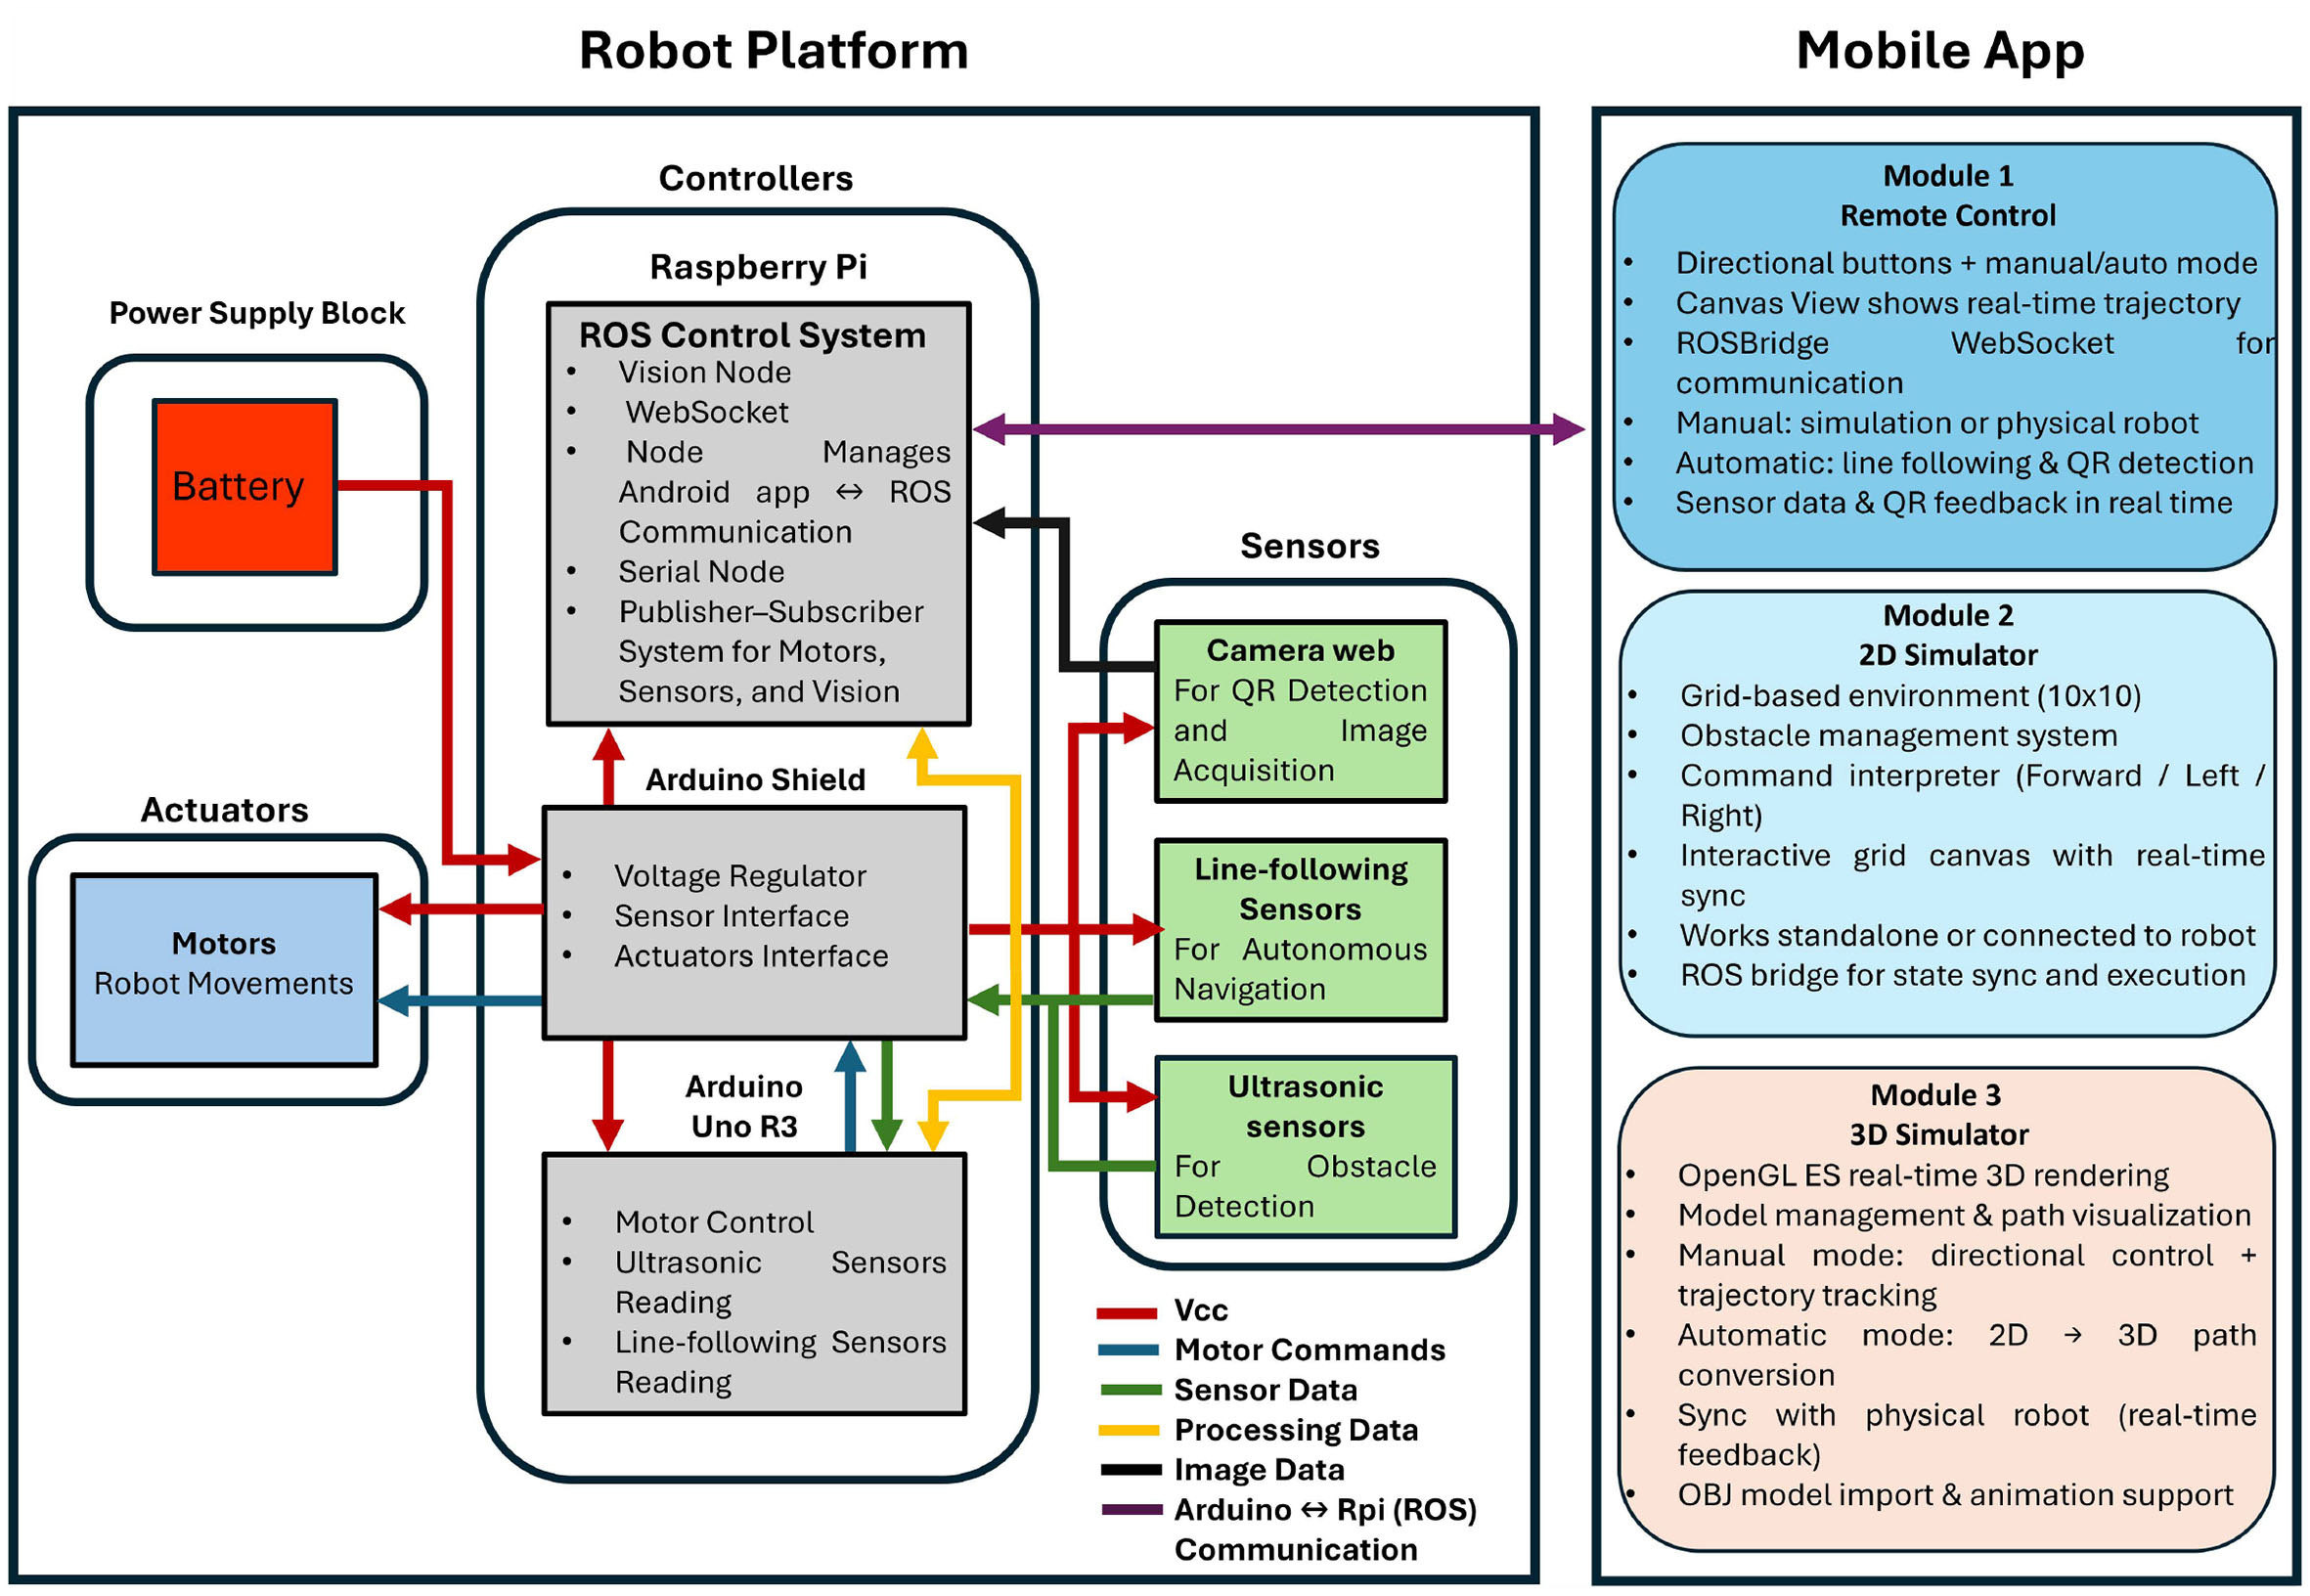
\includegraphics[width=0.6\linewidth]{2026_Mobile2D-3D-RoboticSim/figs/1-s2.0-S235271102500439X-gr1_lrg.jpg}
\end{center}

\end{block} 
\end{frame}


\begin{frame}{\citetitle{\EntradaBibtex} (3)}
\begin{columns}
\begin{column}{0.40\textwidth}
Simulador 2D

\begin{itemize}
		\item  Entorno basado en una cuadrícula 10 × 10.
		\item  El usuario define comandos de movimiento.
		\item  Permite colocar obstáculos.
		\item  Simula la evasión de obstáculos.
		\item  Puede funcionar con o sin robot físico.
	\end{itemize}
\end{column}
\begin{column}{0.60\textwidth}  
\begin{center}
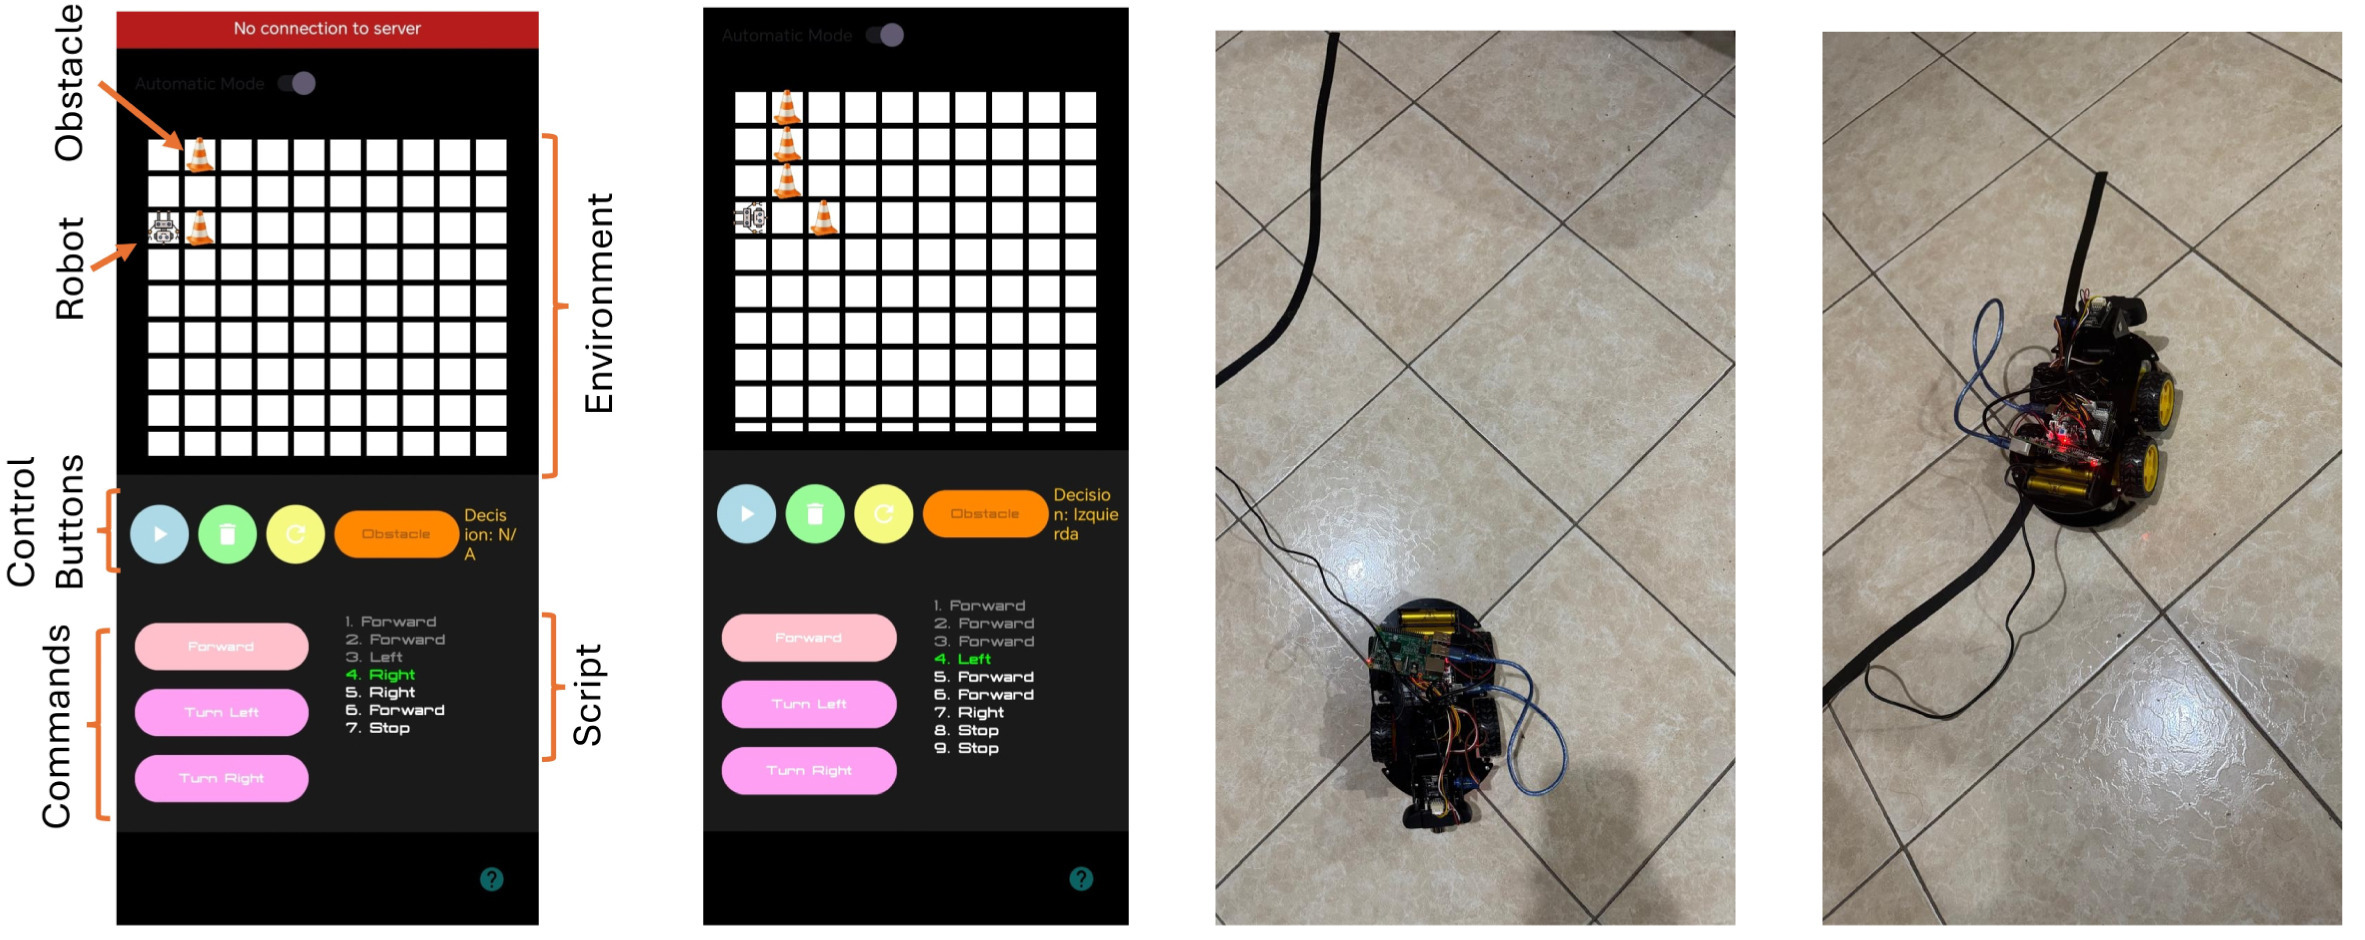
\includegraphics[width=0.98\textwidth]{2026_Mobile2D-3D-RoboticSim/figs/1-s2.0-S235271102500439X-gr4_lrg.jpg}
\end{center}
\end{column} 
\end{columns} 
\end{frame}


\begin{frame}{\citetitle{\EntradaBibtex} (4)}
\begin{columns}
\begin{column}{0.40\textwidth}
Simulador 3D
\begin{itemize}
\item Modelo tridimensional del robot.
\item Visualización de trayectorias.
\item Modos manual y automático.
\item Conversión de rutas 2D a trayectorias 3D.
\item Sincronización con el robot físico.
	\end{itemize}
\end{column}
\begin{column}{0.60\textwidth}  
\begin{center}
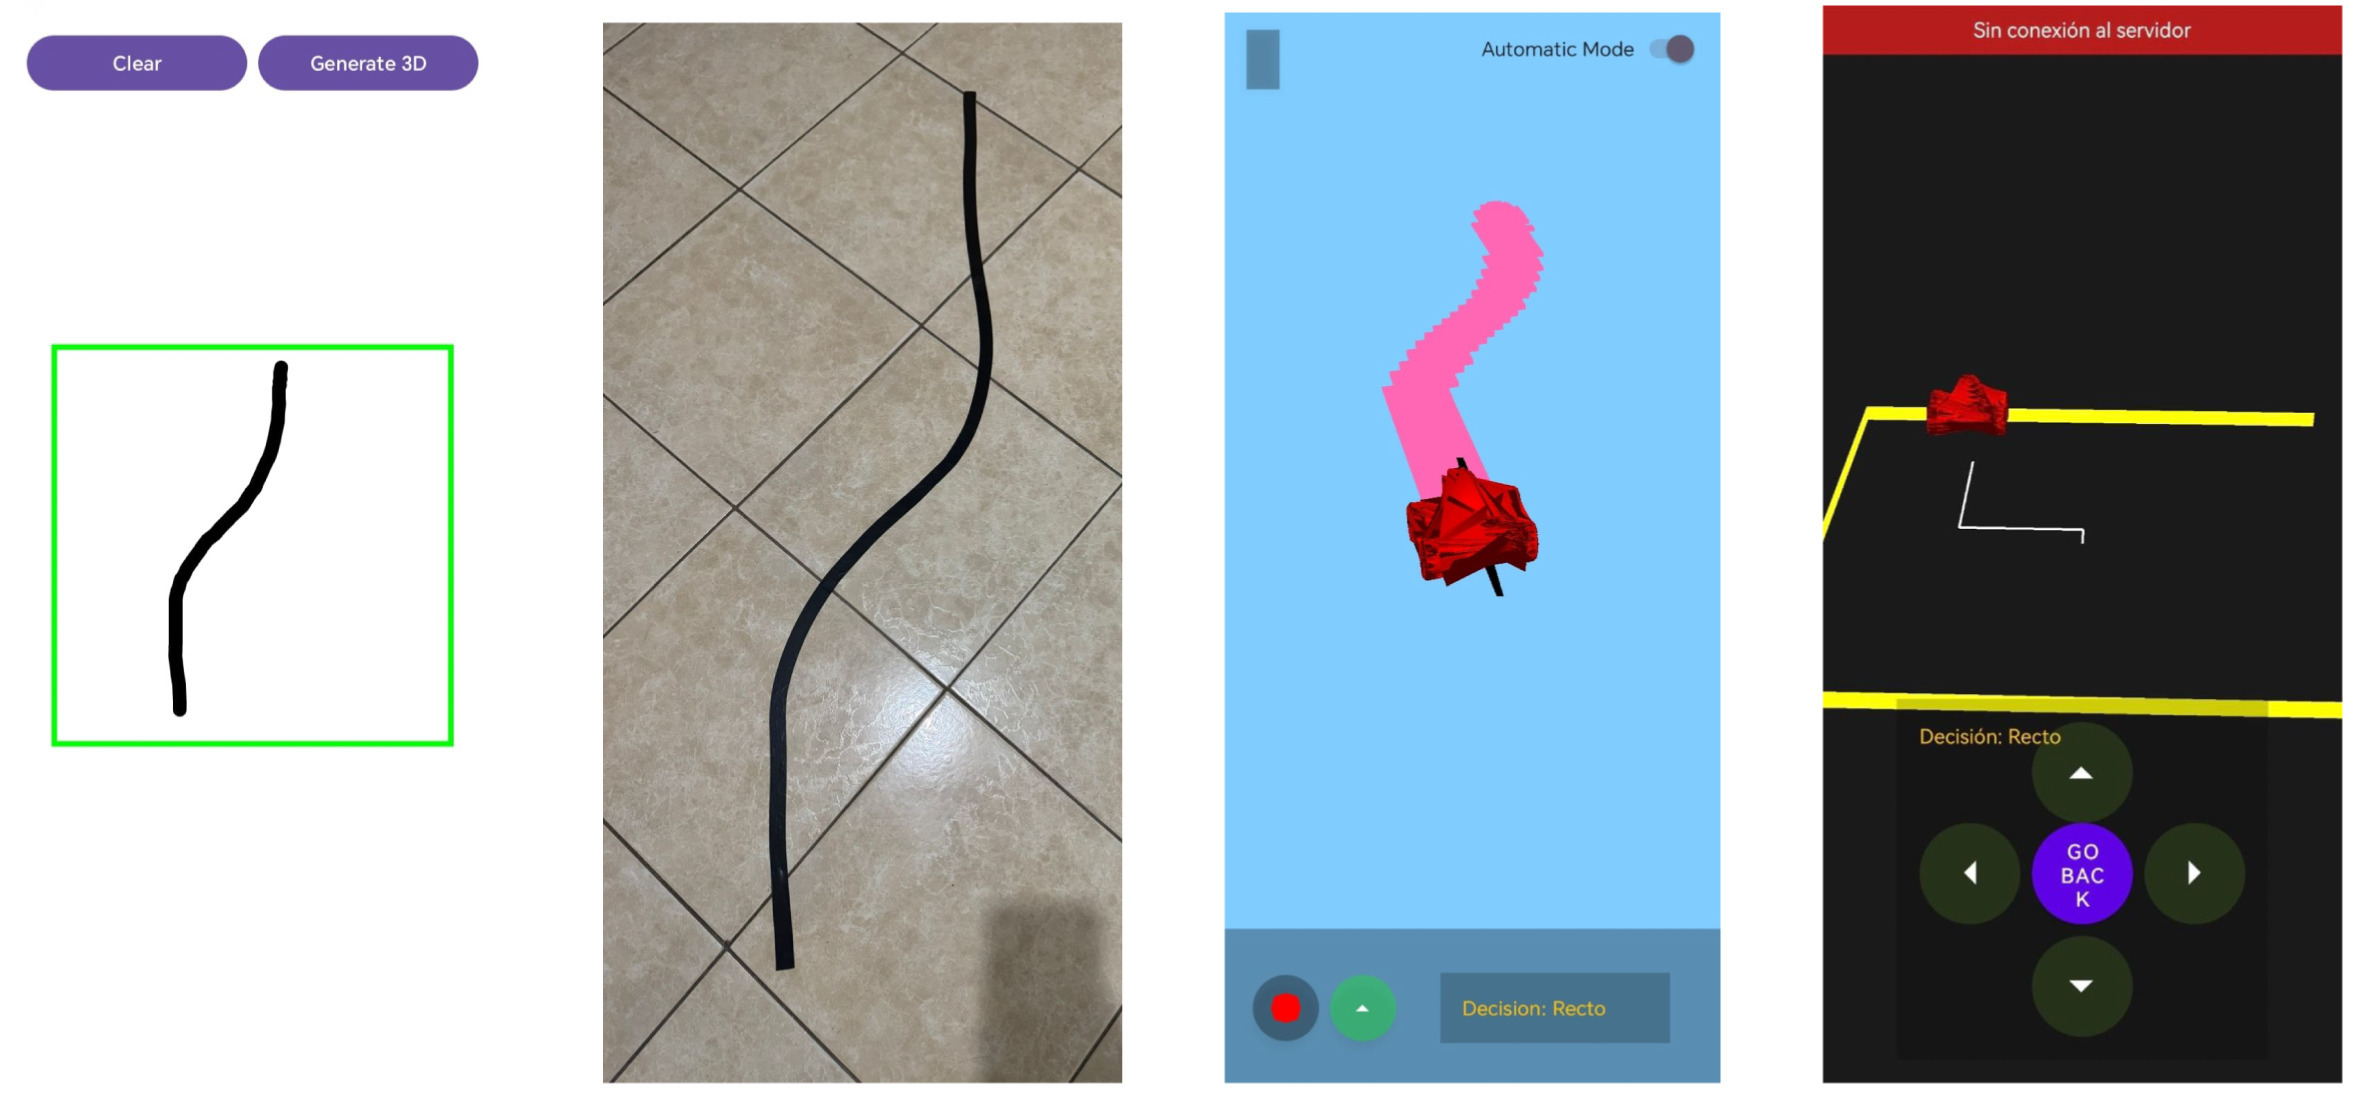
\includegraphics[width=0.98\textwidth]{2026_Mobile2D-3D-RoboticSim/figs/1-s2.0-S235271102500439X-gr5_lrg.jpg}
\end{center}
\end{column} 
\end{columns} 
\end{frame}

\begin{frame}{\citetitle{\EntradaBibtex} (5)}
\begin{block}{Conclusiones} 
Una plataforma híbrida para STEM/STEAM cuyas principales aportaciones son:
\begin{itemize}
\item Plataforma robótica de bajo costo.
\item Integración de robot físico + simulación 2D + simulación 3D.
\item Uso desde dispositivos móviles.
\item Posibilidad de trabajar incluso cuando el robot físico no está disponible.
\item Sincronización entre el mundo virtual y el físico.
\item Aplicación potencial para desarrollar y evaluar pensamiento computacional.
\end{itemize}
Trabajo futuro:
\begin{itemize}
\item Incorporar sensores adicionales.
\item Mejorar la percepción del entorno.
\item Transmitir video en tiempo real desde el robot.
\end{itemize}
\end{block}
\end{frame}
